\chapter{Implementation Timeline}
\section{Overall Planning}

\begin{figure}[h!]
    \centering
    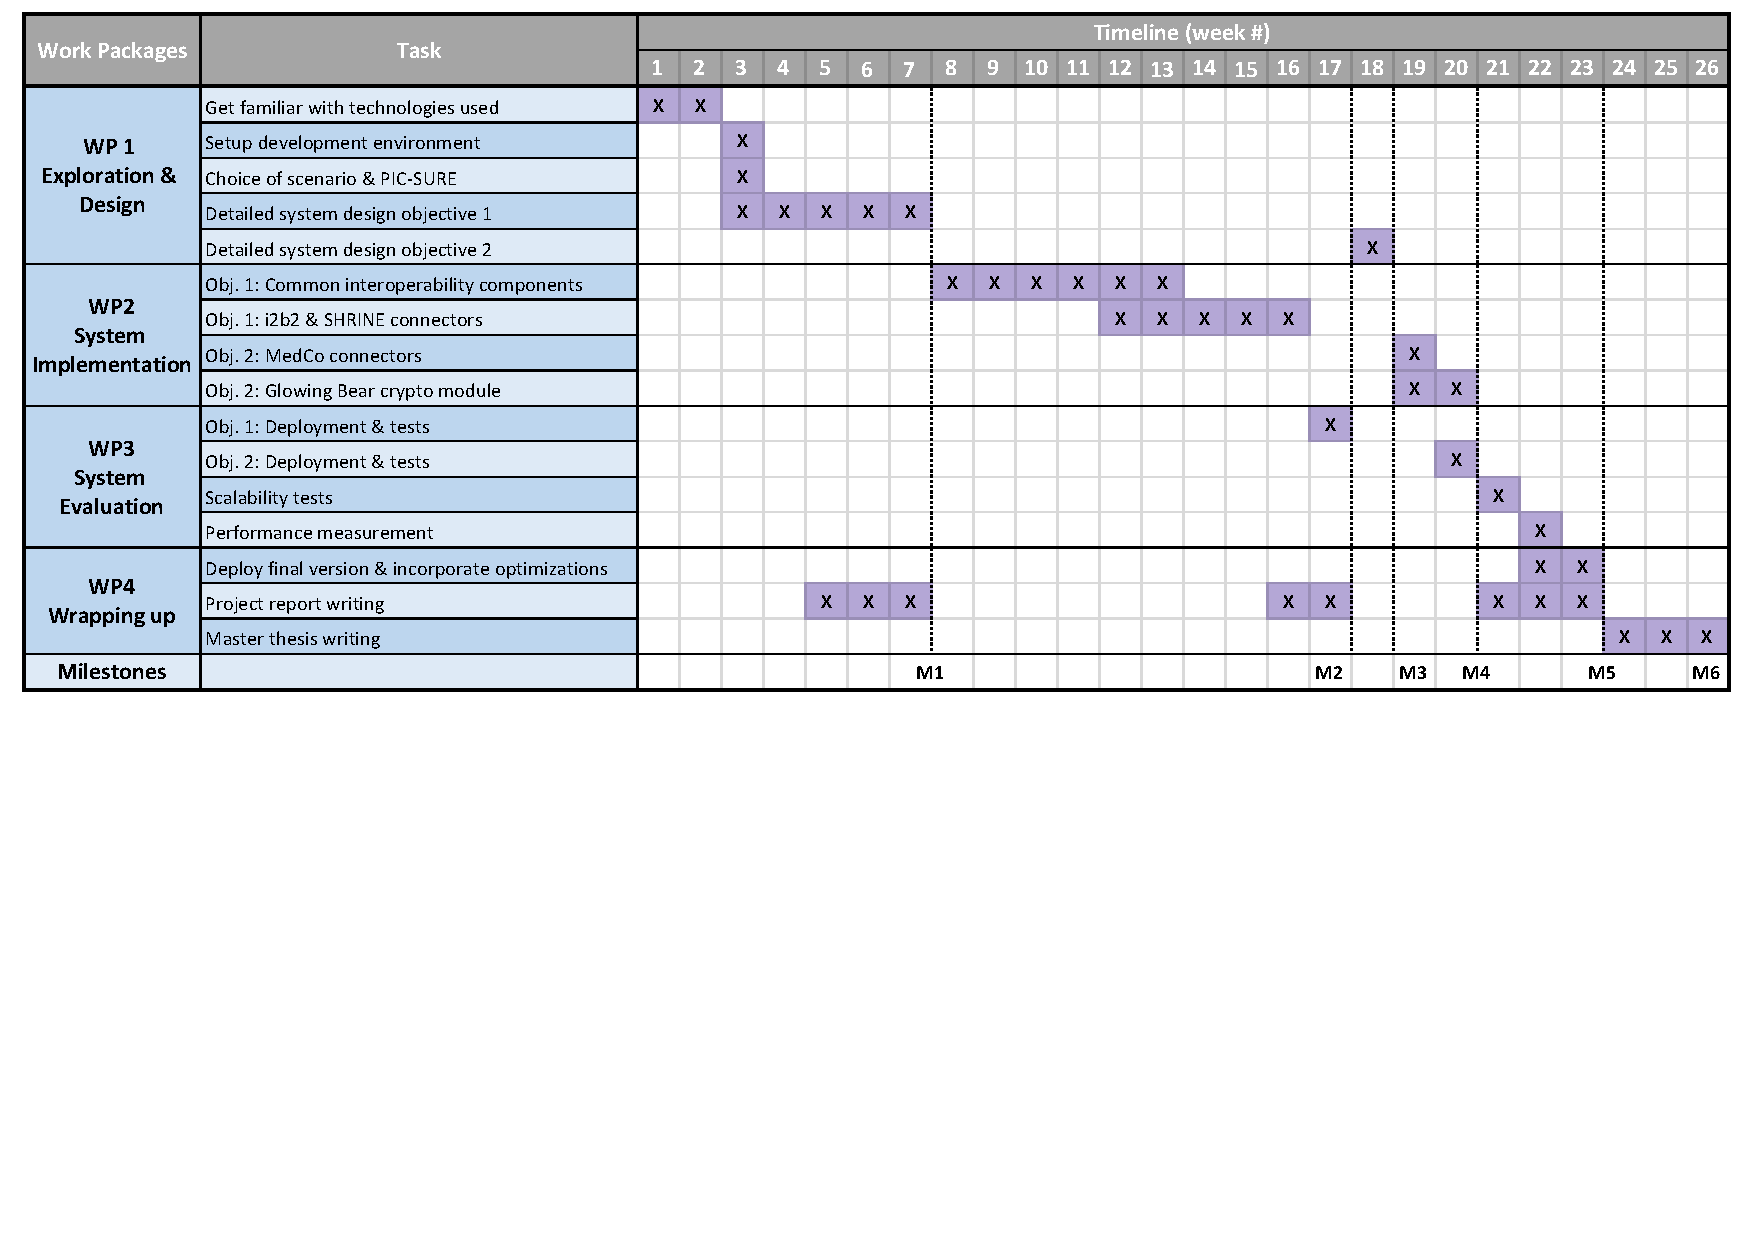
\includegraphics[width=1\textwidth,trim={0 9cm 0 0},clip]{figures/gantt_chartt_v2.pdf}
    \caption{Gantt Chart of Planning v2 (updated at M1)}
    \label{fig:overallplanning}
\end{figure}


\section{Objective 1: Interoperability Layer}

The timeline aims to have first a working system with Glowing Bear, IRCT and i2b2 by taking an horizontal approach, i.e. have each feature working end-to-end individually.
Then the different resources are made to be working with the system.
Total of the implementation of objective 1 is 10 weeks, that are detailed in the breakdown.

\begin{itemize}
    \item System initialization (login, resource list, etc.): \emph{2w}
    \begin{itemize}
        \item Setup: i2b2 + IRCT + keycloak deployment
        \item IRCT resource: i2b2 resource declaration
        \item Glowing Bear: \verb|IRCTResourceService|, configuration
        \item IRCT: small modification for OIDC support
        \item i2b2: OIDC support modification of PM cell
    \end{itemize}
    
    \item Concepts Tree: \emph{1w}
    \begin{itemize}
        \item Glowing Bear: PIC-SURE modifications
        \item IRCT resource: i2b2 tree browsing
    \end{itemize}
    
    \item Query Step 1: Constraints and Aggregates: \emph{2w}
    \begin{itemize}
        \item Glowing Bear: \emph{where} clauses construction
        \item IRCT resource: i2b2 constraints
        \item Glowing Bear: aggregate queries
        \item IRCT resource: i2b2 aggregate queries
    \end{itemize}
    
    % todo: rename data selection to variables selection
    \item Query Step 2: Variables Selection: \emph{0.5w}
    \begin{itemize}
        \item Glowing Bear: \emph{select} clauses construction
        \item IRCT resource: i2b2 variables selection
    \end{itemize}
    
    \item Query Saving: \emph{0.5w}
    \begin{itemize}
        \item IRCT core modification: add missing API calls
        \item IRCT core modification: query per user
        \item Glowing Bear: PIC-SURE modifications
    \end{itemize}
    
    \item Query Step 3: Data Export: \emph{1w}
    \begin{itemize}
        \item Glowing Bear: PIC-SURE modifications
        \item IRCT core modification: add zip file type
        \item IRCT resource: i2b2 result export
    \end{itemize}

    \item IRCT resource: tranSMART 17.1: \emph{2w}
    \begin{itemize}
        \item Setup: tranSMART 17.1 deployment
        \item Modification for OIDC support
        \item Concepts tree browsing
        \item Constraints and Aggregates
        \item Variables selection
        \item Data export
    \end{itemize}
    
    \item IRCT resource: SHRINE: \emph{1w}
    \begin{itemize}
        \item Setup: SHRINE deployment
        \item IRCT resource: extend i2b2, make SHRINE-specific modifications
    \end{itemize}
\end{itemize}
